
\section{Introducción}

\begin{frame}
\frametitle{Ajedrez}
\begin{columns}
    \begin{column}{0.35\textwidth}
        \begin{itemize}
            \item Dos jugadores
            \item Suma cero
        \end{itemize}
    \end{column}
    \begin{column}{0.62\textwidth}
        \newchessgame
        \chessboard[showmover=false]
    \end{column}
\end{columns}
\end{frame}

\begin{frame}
\frametitle{Humano vs. Computadora}
\begin{columns}
    \begin{column}{0.2\textwidth}
        \newchessgame
        \chessboard[showmover=false,boardfontsize=10pt,hlabel=false,vlabel=false]
    \end{column}
    \begin{column}{0.8\textwidth}
        \begin{figure}
            \centering
            \visible<2->{\subfloat{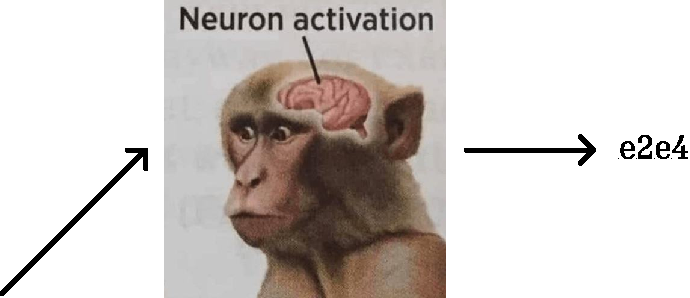
\includegraphics[width=0.8\linewidth]{../assets/slides/human.pdf}}}

            \visible<3->{\subfloat{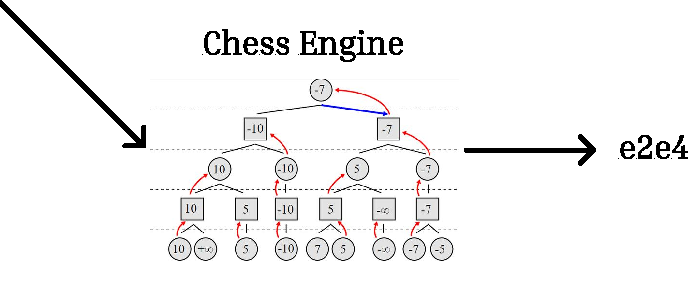
\includegraphics[width=0.8\linewidth]{../assets/slides/computer.pdf}}}
        \end{figure}
    \end{column}
\end{columns}
\end{frame}

\begin{frame}
\frametitle{Ajedrez como árbol}
\begin{figure}
    \centering
    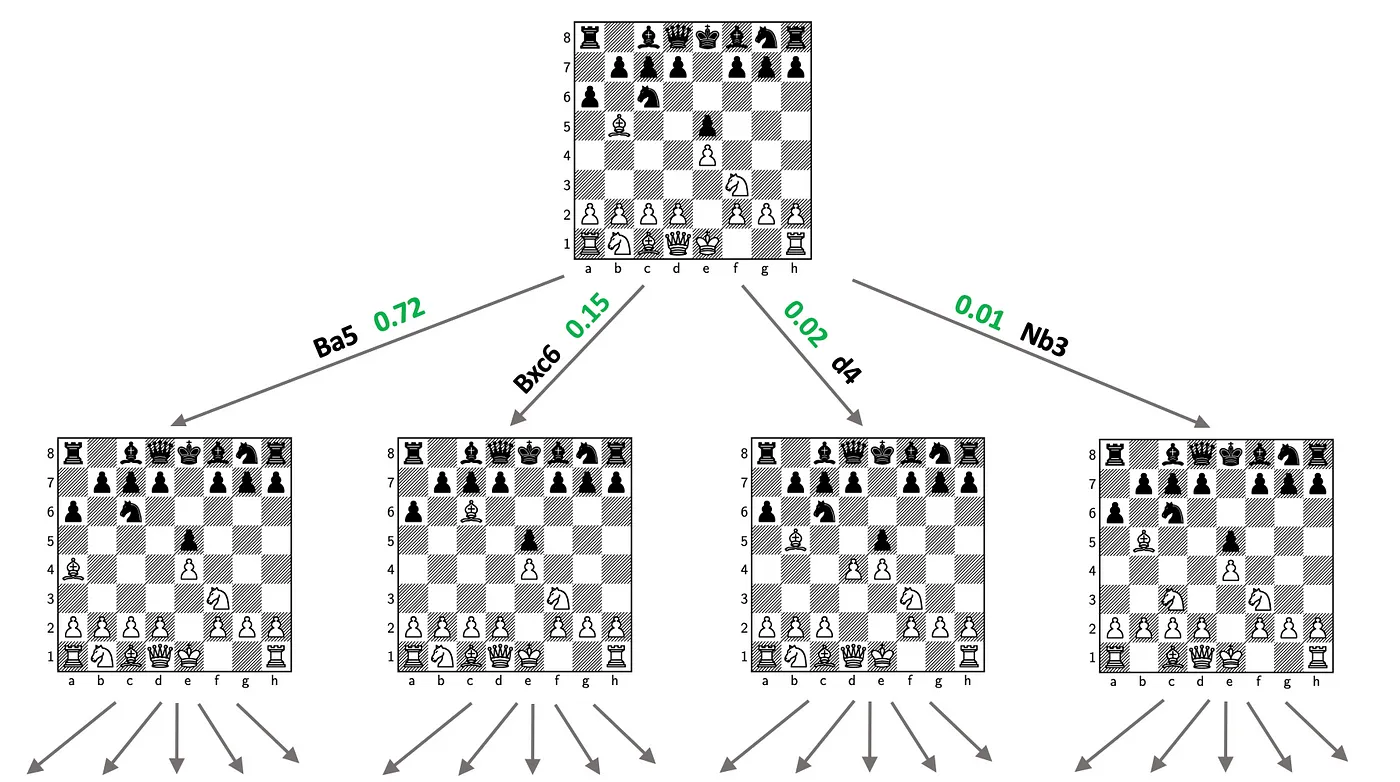
\includegraphics[width=1.0\linewidth]{../assets/slides/chess_tree.png}
\end{figure}
\end{frame}

\begin{frame}
\frametitle{Motores de ajedrez (Chess Engines)}
\begin{columns}
    \begin{column}{0.5\textwidth}
        \begin{itemize}
            \item<1-> Exploran el árbol de juego (Minimax, MCTS, etc.)
            \item<2-> Utilizan funciones de evaluación en las hojas
            \item<3-> La evaluación se propaga hacia arriba, según el algoritmo
        \end{itemize}
    \end{column}
    \begin{column}{0.6\textwidth}
        \begin{figure}
            \centering
            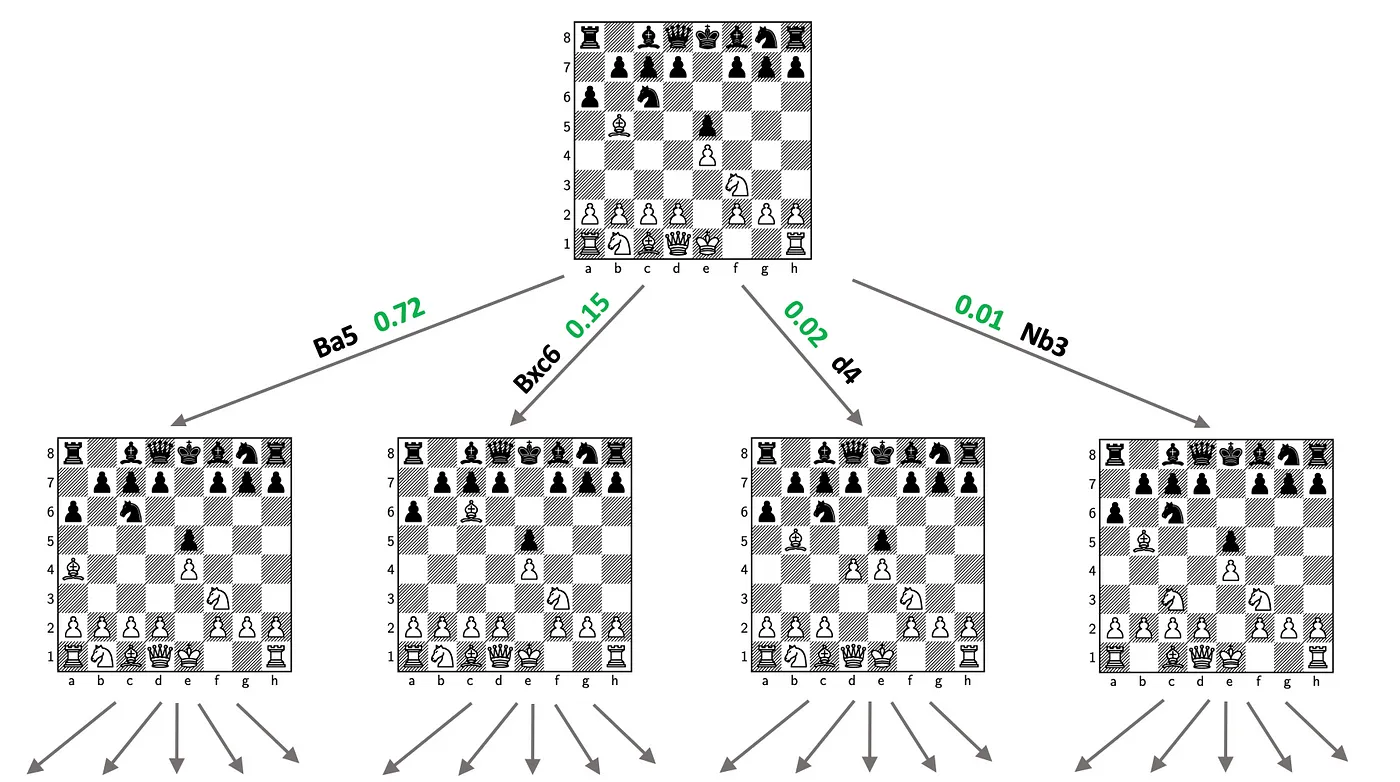
\includegraphics[width=0.9\linewidth]{../assets/slides/chess_tree.png}
        \end{figure}
    \end{column}
\end{columns}
\end{frame}

\begin{frame}
\frametitle{Función de evaluación o \enquote{eval}}
\begin{figure}
    \centering
    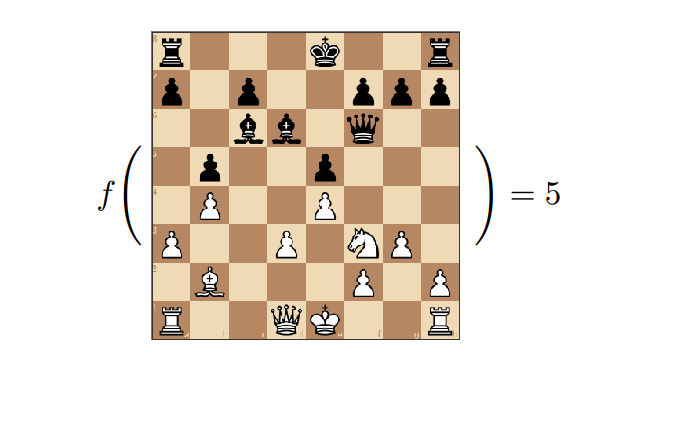
\includegraphics[width=0.8\linewidth]{../assets/slides/eval.png}
\end{figure}
\begin{center}
Intentan resumir todo el subárbol en un solo número. \\
En general son creadas \textit{artesanalmente}
\end{center}
\end{frame}

\begin{frame}
\frametitle{(adelanto) Feature sets: ¿Cómo transformar la posición a un vector para usar NNs?}
\begin{figure}
\centering
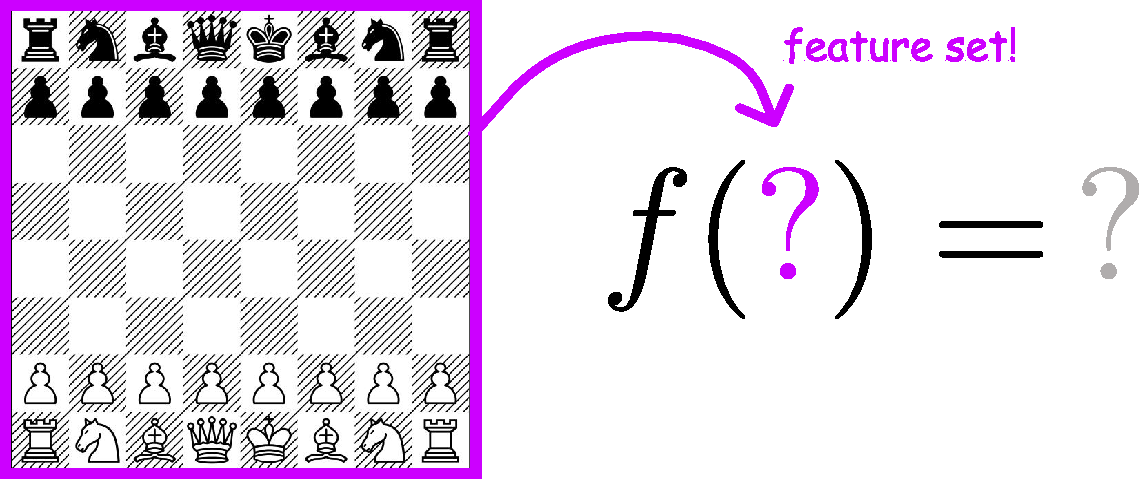
\includegraphics[width=1.0\linewidth]{../assets/slides/fs_motiv2.pdf}
\end{figure}
\end{frame}

\begin{frame}
\frametitle{Motores de ajedrez (breve historia)}
\begin{itemize}
    \item<1-> \textbf{1950s}: Se desarrollan los primeros \textit{algoritmos} de ajedrez
    \item<2-> \textbf{1960s+}: Aparecen los primeros \textit{motores de ajedrez}, lentos y débiles
    \item<3-> \textbf{1997} (hito): IBM DeepMind vence a Garry Kasparov en un torneo
    \item<4-> \textbf{2017 y 2018}: Google DeepMind publica AlphaGo Zero y su sucesor AlphaZero
    \begin{itemize}
        \item se reemplaza la función de evaluación por una red neuronal
    \end{itemize}
    \item<5-> \textbf{2018}: Yu Nasu introduce las redes \reflectbox{NNUE} para Shogi
    \item<6-> \textbf{2020}: Stockfish 12 introduce redes \reflectbox{NNUE} en su evaluación
    \begin{itemize}
        \item se utilizan a la par de evaluaciones artesanales
    \end{itemize}
    \item<7-> \textbf{2024}: Stockfish 16.1 elimina todo aspecto humano de su evaluación, todo es mediante redes neuronales
\end{itemize}
\end{frame}

\begin{frame}
\frametitle{Plan de la tesis}
El objetivo principal es \textbf{proponer y evaluar novedosos feature sets}. \pause Además, \textbf{probar una técnica de entrenamiento} no convencional. \\
\pause
\vspace{1em}
El plan de la presentación es el siguiente:
\begin{itemize}
\item<3-> Implementación de un motor de ajedrez clásico
\item<4-> Definición y ejemplos de feature sets
\item<5-> NNUEs
\item<6-> Entrenamiento de las redes
\item<7-> Experimentos
\end{itemize}
\end{frame}

% \begin{frame}{Contenido}
% \tableofcontents
% \end{frame}
